\chapter{Software Developed}
\label{chapter:software_developed}
Simultaneously with the development of the hardware logic components there was software developed. During this project first it was developed a software for communication with the \textit{IOb-SoC} through serial. Second it was developed a new hardware simulation software. Thirdly, firmware that could test and run interrupt routines was developed. Fourth, the needed software/firmware to execute an \acrlong{os} was adapted and compiled for the \acrshort{soc} developed. Finally, there were multiple Makefiles written that facilitate the user interaction and further development.

Some of the software developed was not mandatory to get a full-fledged \acrlong{os} to work with the \acrlong{soc} designed. The complementary software was matured because it facilitates the project development. Furthermore, the additional software allows the \textit{IOb-SoC} platform to support more features.

In this chapter the software developed will be analyzed. The new \textit{Python} \textit{Console} and the new simulation system were already implemented on the upstream \textit{IOb-SoC} template. This software is already being used by other developers. Moreover, it has been improved by the \textit{IObundle} developers using it.

\section{\textit{Python} \textit{Console}}
\label{section:pyhton_console}
The \textit{Console} is a program that runs on the user computer and communicates with the board where the \textit{IOb-SoC} is implemented using an \textit{RS-232} connection. Initially the \textit{IOb-SoC} had a \textit{Console} written in \textit{C} programming language. One of the first tasks developed was the translation of the \textit{Console} program to \textit{Python}.

The \textit{C} \textit{Console} makes use of a set of functions on a independent file that were written to read/write to the serial port. The \textit{Python} program uses the \textit{PySerial} library, which provides ready-made communication functions like those in the original \textit{C} code. Using \textit{PySerial} is better because the community regularly maintains and updates \textit{PySerial}. \textit{PySerial} provides additional features, is less prone to have bugs, and the communication is more trustworthy comparing with the \textit{C} functions.

One of the reasons to translate the \textit{Console} program was to integrate an existing Ethernet controller already written in \textit{Python}. \textit{Python} can easily exploit feature like files, sockets and other \acrfull{os} functionalities.

The \textit{Python} \textit{Console} program can be used in two different modes: locally working with simulators, or communicating with a board running \textit{IOb-SoC}. The program mode can be choose when calling the \textit{Console} through adding \enquote{-L} or \enquote{--local} to the invoking arguments. This is an alteration to the original \textit{Console} program. The \textit{C} \textit{Console} could only works with the \acrshort{fpga} board. When the \textit{Console} is run in board mode a physical implementation of \textit{IOb-SoC} runs on the board and communicates with \textit{Console} through a \textit{RS-232} serial connection. If the \textit{Console} is called with the \enquote{-L} or \enquote{--local} augment it will communicate with the simulator. The communication with the hardware simulation is identical to the one with the board. They exchange the same messages. When communicating with the simulator the \textit{Console} uses files to send and receive data from the \textit{IOb-SoC} hardware simulation. The \textit{Console} program when stating creates two empty files in the simulation directory. The \enquote{cnsl2soc} is used to send messages from the \textit{Console} to the \acrshort{soc}. The \enquote{soc2cnsl} is used by the \textit{Console} to receive messages from the \acrshort{soc}. Both files only contain one byte at a time. The fact if the files are empty or not is used to synchronize the simulation with the \textit{Console}. After reading from one of the files the simulation or the \textit{Console} program has to empty the respective file.

The way the code is structured is very similar to how it was on the \textit{C} \textit{Console} program. It starts by defining the parameters that influence messages identifiers and serial communication (for example, the number of bits per byte, the parity and the number of stop bits). When the program enters its primary function, it starts a loop where it waits for an available byte to read, either from the serial port or the file, depending on the mode the \textit{Console} was called. After receiving the byte from the \acrshort{soc}, it computes what type of message it is. The program exits successfully if the byte received is an \acrlong{eot} (\acrshort{eot} = 04, \acrshort{ascii} value in hexadecimal). If the byte received is an \acrlong{enq} (\acrshort{enq} = 05, \acrshort{ascii} value in hexadecimal), the program checks if it was the first time it received an enquiry. If it was, it could have one of either behavior: if the program was called with an argument equivalent to \enquote{-f}, meaning that there is a firmware that should be uploaded to the \textit{IOb-SoC}, the \textit{Console} sends a \textit{Send a file request} message (FRX = 08, value in hexadecimal) to the \textit{IOb-SoC}; if there is not a firmware file to send then the \textit{Console} responds to the \textit{IOb-SoC} with an \acrlong{ack} (\acrshort{ack} = 06, \acrshort{ascii} value in hexadecimal). If the \textit{Console} receives a Receive a file request message (FTX = 07, value in hexadecimal), it will run a function that will receive any file sent from the \textit{IOb-SoC} to the computer and save it under the directory where it is running. If the \textit{Console} receives a \textit{Send a file request} message, it will run a function that will send any file requested from the \textit{IOb-SoC} to it. Any other byte received will be printed onto the stdout.

The FRX and the FTX bytes are specific to the \textit{IOb-SoC} platform software. This could cause a problem when using external software that does not attribute the same meaning to their respective values. To solve this problem a meaning for the \acrlong{dc1} (\acrshort{dc1} = 11, \acrshort{ascii} value in hexadecimal) byte was created. When receiving a \acrshort{dc1} byte the \textit{Console} deactivates all platform specific meanings for the respective bytes. This means that after receiving a \acrshort{dc1} byte stops associating the value 0x07, 0x08, 0x11 to FTX, FRX and \acrshort{dc1} respectively.

An example of how to call the \textit{Console} to communicate with the simulation and send the firmware to the \textit{IOb-SoC} when it starts would be \ref{lst:call_console}. The \enquote{\&} at the end means that the \textit{Console} program is going to run in the background. Allowing to run other programs while the \textit{Console} executes.

\begin{lstlisting}[language=make, caption={Call \textit{Console} program}, label=lst:call_console]
    CONSOLE_CMD=$(CONSOLE_DIRECTORY)/console -L -f &
\end{lstlisting}

\section{\textit{IOb-SoC} Simulation}
\label{section:simulation}
In order to support the new \textit{Console} simulation mode a new \textit{IOb-SoC} verification mechanism had to be developed. Verification is one an important topic when developing hardware. A correct and precise verification saves time since the hardware does not have to be synthesized and flashed to an FPGA every time an SoC designer wants to test a new feature.

The original simulation \textbf{How it worked}... The responses given to the \textit{IOb-SoC} were performed with a emulation of the \textit{Console} program written in Verilog. Every time the \textit{Console} was updated, the simulation \textit{Console} also had to be updated. Hence, the idea was to create a testbench that allowed the simulator to interact with the \textit{Console} program. The new simulation now has the advantage of mostly using the same \textit{Console} program as when the \textit{IOb-SoC} is implemented in a \acrshort{fpga}.

\subsection{UUT Top Hardware module}
This top module creates a \textit{verilog} wrapper of the \acrfull{uut} that allows it to interact with the different hardware logic simulators. Even tho this is written hardware logic it is never implemented as real hardware. This module is only used in simulation as software.

The top module file is an adaptation of the previous \textit{verilog} file used on the Icarus simulation. Previously, the verilog top file would interact directly with the \textit{Console}. Similarly to the new hardware top module an \acrshort{uart} module is instantiated and a serial connection with the \textit{IOb-SoC} is simulated. Although in this project the \textit{IOb-UART} in the \acrfull{soc} was swapped for the \textit{UART16550} in the 

\begin{figure}[!ht]
    \centering
    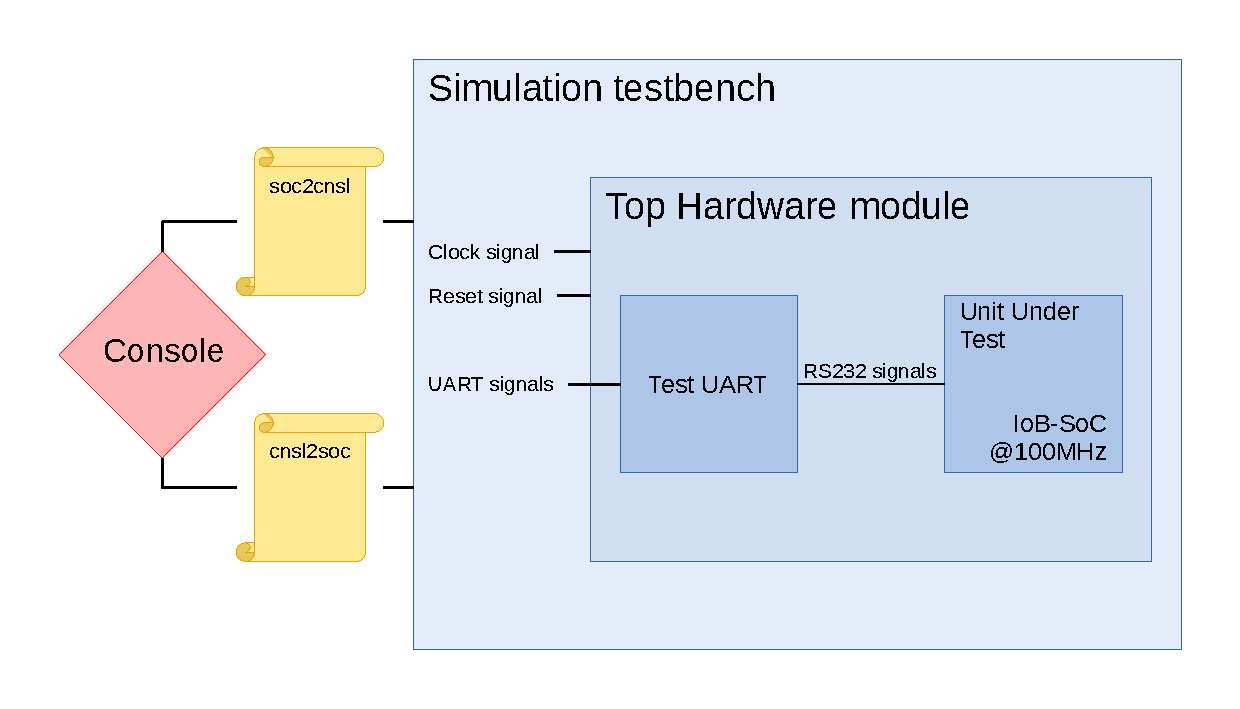
\includegraphics[width=\linewidth]{uut_top_hw.pdf}
    \caption{Simulated hardware interfaces.}
    \label{fig:uut_top_hw}
\end{figure}

\subsection{Verilator Testbench}
Verilator transforms the Verilog HDL designs into a C++ program that can be executed after being compiled. Using C++ to create a testbench permits to execute the converted hardware program simulating the hardware initially described in Verilog. While also allowing to easily make use of system calls. The testbench needed to run with Verilator is similar to the testbench in Verilog used with Icarus.
%Tabela comparativa entre icarus e verilator

\section{Interrupt Routine}
\label{section:barebones_interrupt_routine}
During the development of the \acrshort{clint} hardware unit there was no firmware that used the \acrshort{clint}. The \acrshort{clint} enables the support for time or software related interrupt. Therefor, to test the \acrshort{clint} hardware it was needed to create a simulation testbench. Moreover, to understand how interrupts are used in code and handled by the \acrshort{cpu} a bare-metal firmware that uses interrupts was created.

To generate a time related interrupt the software has to write to the \enquote{MTIMECMP} register. The \enquote{MTIMECMP} register address is the \enquote{MTIMECMP\_BASE} address, which is 0x4000, plus 0x08 times the core id. The core id is the \enquote{TARGET}, \acrshort{cpu} core, that is suppose to receive the interrupt notification. In this project since there is only one core the core id is 0. Furthermore, when writing firmware to run on the \acrshort{soc} it is needed to consider the \acrshort{clint} peripheral base address and add it to the \enquote{MTIMECMP} register address. To make a timer interrupt to trigger after 10 seconds the firmware as to do more than just write to the \enquote{MTIMECMP}. First, the firmware has to read the current time. The current time can be obtained from the \enquote{MTIME} register. Although not directly since the \enquote{MTIME} register increments with the \acrshort{clint} designed frequency, in this case 100MHz. To convert the value in \enquote{MTIME} register to seconds we know that $seconds=\frac{*(MTIME)}{frequency}$. The \enquote{MTIME} register address is obtained similarly to the \enquote{MTIMECMP} register but instead of the \enquote{MTIMECMP\_BASE}, the \enquote{MTIME\_BASE}, which is 0xbff8, is used. After reading the current time, the value that needs to be stored in \enquote{MTIMECMP} register is calculated. The value is calculated by adding the time to wait before the interrupt is triggered to the current time. The value calculated can then be stored in the \enquote{MTIMECMP} register. When the \enquote{MTIME} register value is equal or greater than the \enquote{MTIMECMP} register value the timer interrupt is enabled. The pseudo code to set up the timer interrupt can be seen in the code snippet \ref*{lst:set_up_mtip}. 

\begin{lstlisting}[language=C, caption={Set Up Timer Interrupt.}, label=lst:set_up_mtip]
    #define MTIMECMP_BASE 0x4000
    #define MTIME_BASE 0xbff8
    #define FREQ 100000000
    void set_up_mtip(time_sec){
        int aux_value = 0;
        int core_id = 0;
        aux_value = *(MTIME_BASE+8*core_id)
        aux_value = aux_value + time_sec*FREQ;
        *(MTIMECMP_BASE+8*core_id) = aux_value;
    }
\end{lstlisting}

The core id could have been read from the \acrshort{csr} which saves its value. The RISC-V instruction that does so is \enquote{csrr    \%0, mhartid}. An example of a C code integration would be code snippet \ref*{lst:read_mhartid}.

\begin{lstlisting}[language=C, caption={Read core id from \acrshort{csr}.}, label=lst:read_mhartid]
    static inline uint_32_t csr_read_mhartid(void) {
        uint_32_t value;        
        __asm__ volatile ("csrr    %0, mhartid" 
                          : "=r" (value)  /* output : register */
                          : /* input : none */
                          : /* clobbers: none */);
        return value;
    }
\end{lstlisting}

One of the software interrupt usage is to synchronize various cores in a system. When dividing workload between cores there might be a time when core 1 has to synchronize with core 0. To do this core 1 would wait until core 0 generates a software interrupt targeting core 1. In this project there is only one core so this situation does not occur. But applications can run concurrently with multi threading. One applications could wait until a software interrupt is triggered. This software interrupt could be triggered by another application running in core 0 and targeting core 0. To generate a software related interrupt the software has to write to the \enquote{MSIP} register. The \enquote{MSIP} register address is the \enquote{MSIP\_BASE} address, which is 0x00, plus 0x04 times the core id. When running the firmware adding the \acrshort{clint} peripheral base address to the \enquote{MSIP} register can not be overlooked. The \enquote{MSIP} register can only be written through external sources. The \acrshort{clint} hardware is not able to change it internally. The pseudo code to set up the software interrupt can be seen in the code snippet \ref*{lst:set_up_msip}. 

\begin{lstlisting}[language=C, caption={Set Up Software Interrupt.}, label=lst:set_up_msip]
    #define MSIP_BASE 0x00
    void set_up_msip(){
        int core_id = csr_read_mhartid();
        *(MSIP_BASE+4*core_id) = 1;
    }
\end{lstlisting}

After enabling an interrupt the \acrshort{clint} sends a hardware notification. The interrupts notification has to be handled by the rest of the hardware. The \acrshort{clint} testbench and the bare-metal firmware handle the interrupts notification differently.

\subsection{CLINT simulation}

\subsection{Bare-metal firmware}

\section{IOb-SoC Linux OS integration}
\label{section:linux_os_integration}
Talk about the noncannonical.py

\subsection{Bootloaders}
IOb-SoC Linux Stage 0 Bootloader

OpenSBI

\subsection{Device Tree}

\subsection{Linux kernel}

\subsection{Root File system}

\section{Makefiles}